\documentclass[a4paper,10pt]{IEEEtran}
\usepackage[left=.5in, top=.5in, right=.5in, nohead,nofoot]{geometry} 
\usepackage{float}
\usepackage{graphicx}

%opening
\title{Teaching the Visualization Toolkit by Example}
\author{David Doria}

\begin{document}

\maketitle

\begin{abstract}
The Visualization Toolkit (VTK) is one of the standard choices for developing custom scientific and information visualization solutions. If offers many visualization and data analysis algorithms and an excellent pipeline architecture to string them together. A very typical problem with very large systems such as VTK is that they come with very steep learning curves. In this paper we present the solution we have developed to remedy this problem. We have created a system which helps users map abstract visualization concepts into concrete VTK terminology. Once the appropriate VTK concept is identified, we provide a compilable example of how to use it. This is done in a manner which is robust to the evolving toolkit, as well as takes advantage of existing library documentation. Our system helps new users get started with VTK faster than ever.
\end{abstract}

% \begin{figure}[h]
% \centering
% \includegraphics[width=0.2\linewidth]{saddle}
% \includegraphics[width=0.2\linewidth]{schwartz}
% \end{figure}

%%%%%%%%%%%%%%%%%%
\section{Introduction}
Scientific and information visualization have never been more important. An ever increasing number of scientists and engineers from an expanding number of technical fields require visualization techniques to work with and analyze their data. Many software packages are available to visualize data common to particular fields (e.g. molecule visualization in Chemistry). However, it is not uncommon in scientific research to want to visualize data in a new way or interact with it in a way that is not currently available. For these cases a programmable solution is required. For almost two decades, VTK has provided an excellent platform for experts in visualization to develop new algorithms. Recently, the need to provide non-expert users an enjoyable and efficient experience displaying and interperting their data was recognized. These users are likely also non-expert programmers, so we must provide a way for them to map concepts in visualization (e.g. ``I want to make the sphere red'') to concepts in the library (e.g. \verb|sphereActor->GetProperty()->SetColor(1,0,0);|). We set out to create a system to reduce the barrier of entry to VTK with three goals in mind:
\begin{itemize}
 \item Catering to new users who are non-experts in visualization and non-expert programmers
 \item Hosting the system in such a way that it can be built and edited by the community
 \item Keeping the system up to date as the toolkit evolves
\end{itemize}

%%%%%%%%%%%%%%%%%%
\section{Reasons for Complexity}
Being an open-source project, VTK is mainly developed by researchers who can justify a particular addition to their funding sources. Unfortunately, this often leads to these new features being added without clearly explaining what they do and how to use them.

%%%%%%%%%%%%%%%%%%
\section{Why Do We Want To Reduce The Learning Curve?}
Most new users will decide very quickly if a software package is a good fit for their needs. There are two reasons we want this initial experience with VTK to be a pleasant one. First, with the ever increasing complexity of scientific algorithms, sharing code among fellow researchers is becoming extremely important. VTK provides a common language for algorithms which operate on many types of data, so attracting people to such a language is helps progress many scientific fields. Second, being an open source package, more user directly equates to more potential developers. 

%%%%%%%%%%%%%%%%%%
\section{The Solution - VTK Examples Wiki}
Our solution was to create the VTK Examples Wiki project (http://www.vtk.org/Wiki/VTK/Examples). We have created a wiki with over 500 fully compilable c++ examples (the main language of VTK) and hundreds of examples in wrapped languages (Python, Java, and Tcl) demonstrating how to perform common operations in VTK.

\subsection{Wiki}
The wiki format was chosen because, in the spirit of open-source collaboration, it allows any user to add a new example as they find techniques that are not sufficiently explained elsewhere. The wiki format also has a very low barrier of entry itself. A user can simply click ``edit'', edit the text, and then save the page. No new tools or skills are required to be learned.

\subsection{Reduction in Reduntant Questions on the Mailing List}
We found that the same questions were being asked over and over again on the VTK mailing list. This is terribly inefficient as it uses valuable developer time that could be spent adding new features to answer questions that should be ``obvious''. It is exactly this jump from a concept to a clear and obvious solution that we are attempting to facilitate.

\subsection{Structure of the List of Examples}
For each language supported by VTK there is a separate examples wiki page. Within each language, the examples are broken down into categories. Each category consists of approximately 5 - 25 examples sharing a common theme. For example, two categories are ``File Input and Output'' and ``Geometric Objects''. Within each of these categories, the individual examples are arranged in a table consisting of columns titled ``Example Name'', ``VTK Classes Demonstrated'', and ``Description''. This table is sortable, so the user can more easily find what they are looking for either by concept description or VTK class name.

\subsection{Searching the Wiki}
The wiki is searchable in two ways. The first, and most important for new users, is the map from visualization concept $\rightarrow$ VTK class. The second search technique, which becomes increasingly important as a user starts to gain experience with VTK, is VTK class/concept $\rightarrow$ demonstration/example.
\subsubsection{General Concept to VTK Terminology Mapping}
Users seeking answers to questions such as, "How do I add color to my data?", "How do I move the camera?", and "How do I compute the area of a triangle?" can search the wiki for these types of ``common language'' terms. For example, a search for ``triangle area'' will bring a user to an example which creates a triangle and shows how to compute the area.
\subsubsection{Searching for VTK Terminology Directly}
Users who want to know ``I saw that there is a class called vtkKdTree. This sounds like what I want - how do I use it?'' can simply search the wiki for ``vtkKdTree'' to find all of the examples that demonstrate techniques involving K-D Trees.

\subsection{Relationship to Documentation}
VTK uses Doxygen to generate documentation directly from comments in the code. This documentation is very helpful to an experienced user, but a new user may feel overwhelmed by the sheer volume of classes and functions that are available. To ensure the best information is always easily accessible, we provide links from the documentation to the Wiki Examples, as well as links from the Wiki Examples to the documentation.

\subsection{Structure of an Example}
\begin{itemize}
 \item Description
 \item Output
 \item VTK Classes Demonstrated
 \item ExampleName.cxx
 \item CMakeLists.txt
\end{itemize}


%%%%%%%%%%%%%%%%%%%
\section{Regression Testing}
VTK is constantly changing and improving. An example of how to use VTK last month may not still be valid. Therefore, we decided that the examples must be compiled nightly, and they must be tested to verify that they still produce correct results.

\subsection{Scraping the Wiki}
As mentioned earlier, examples can be added and modified directly on the wiki. Unfortunately, this does not provide an easy environment in which to compile and test code. To remedy this, we must convert the wiki into a standard files (.cxx and .txt). To do this, we have written a script which ``crawls'' the wiki looking for examples. When it finds one, it parses the page and downloads the content of the .cxx and .txt file to normal text files on the server.

\subsection{Archival and Revision Control in a Git Repository}
While the wiki has its own version of revision control, we prefer to rely on a more standard revision control system, Git. Each night after the wiki is scraped, the resulting files are pushed to a git repository. This serves a dual purpose. First, it is a backup/archive of the entire set of examples. Second, it allows more serious users to download all of the examples at once, allowing them the flexibility of using their own searching tools as they now have the examples in a standard programming file format.

\subsection{Testing Framework}
VTK uses CMake as its build system. A powerful tool that comes with CMake is CTest. CTest simply takes a file that is structured identically to a standard c++ file, but with \verb|main()| replaced with \verb|TestName()|. Since we want users to be able to use the examples from the wiki directly, the examples on the wiki must use \verb|main()|. To allow for this, we have written a script which changes \verb|main()| to \verb|TestName()| automatically.

\subsection{Baseline Images}
To test that the example still produces the intended output, when the example is added, the creator must verify that the output produced by the example at the time that it is added is correct. To do this, the Testing Framework automatically saves the output that is displayed on the screen to a file. The creator of the example must verify that the output image looks correct, and then add it to the \verb|Examples/Baseline| folder. This baseline image is automatically uploaded onto the wiki each night during the scraping process. This has a built in bonus of also providing the user an image of what they should expect to see upon compiling and running the examples themselves!

\section{Example}
\begin{itemize}
\item \bf{Example name:} TriangulateTerrainMap
\item \bf{VTK Classes Demonstrated:} vtkDelaunay2D
\item \bf{Description:} Generate heights (z values) on a 10x10 grid (a terrain map) and then triangulate the points to form a surface.
\item \bf{Output:}
\begin{figure}[H]
   \centering
   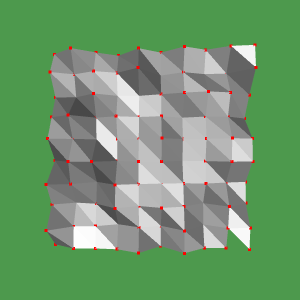
\includegraphics[width=0.4\linewidth]{TriangulateTerrainMap}
   \caption{Triangulated Terrain Map}
\end{figure}

\item 
\begin{verbatim}
   // Triangulate the grid points
  vtkSmartPointer<vtkDelaunay2D> delaunay =
    vtkSmartPointer<vtkDelaunay2D>::New();
  delaunay->SetInput(polydata);
  delaunay->Update();
 
  // Create a mapper and actor
  vtkSmartPointer<vtkPolyDataMapper> triangulatedMapper =
    vtkSmartPointer<vtkPolyDataMapper>::New();
  triangulatedMapper->SetInputConnection(delaunay->GetOutputPort());
\end{verbatim}
\end{itemize}




%%%%%%%%%%%%%%%%%%%
\section{Conclusion}
If you have left VTK because it was too hard to learn, we invite you to give it another try now that the examples wiki is up and running! If you are new to visualization and scientific computing and would like to learn by example, you have come to the right place!
\end{document}
